\section{Model}
\numberwithin{equation}{section}

The calculation of the ASE Flux $\Phi_{ASE}$ model is based on the concept of an
active gain medium with planar top and bottom surfaces. This \emph{gain medium} is
then sampled and for each \emph{sample point} (Figure
\ref{graphic:samples_reduced}) the amplification of spontaneous emission is
determined. 


\subsection{Monte Carlo simulation}
\label{subsec:monteCarlo}

For a given sample point $s_i$ in the gain medium, $\Phi_{ASE}$ can
be calculated as described in \cite{ASE2010}:
\begin{equation}
  \label{eq:phi_ase_daniel} 
  \Phi_{ASE}(s_i)=\frac{1}{4\pi}\iint\limits_{V \lambda}
  \frac
    {\hat{n}(r)}
    {\tau_{f}|\rho(r,s_i)|^2}
  ~g(\lambda)
  ~G_{r\rightarrow s_i}
  ~dV d\lambda
\end{equation}
where $G_{r\rightarrow s_i}$ denotes the amplification between
position $r$ and $s_i$ as a line integral on the vector
$\overrightarrow{rs_i}$.  One approach to solve the integral is to use Monte
Carlo integration. For a single wavelenght, the equation is rewritten as a sum:
\begin{equation}
  \label{eq:monte_carlo_ase}
  \Phi_{ASE}(s_i) = 
  \frac{1}{4\pi N\tau_f}
  \sum^{N-1}_{u=0} \hat{n}(r_{i,u}) \cdot gain(\overrightarrow{r_{i,u}s_i})
\end{equation}
where $N$ is the number of Monte Carlo simulations (the number of \emph{rays}
simulated) and $gain(\overrightarrow{r_{i,u}s_i})$ is the amplification along the
path $\overrightarrow{r_{i,u}s_i}$ of a single ray as it will be described in
formula \eqref{eq:gain}. 


\subsection{The gain medium mesh} \label{subsec:meshSampling}

In order to distribute the sample points on the medium, it is treated as
a horizontal 2-dimensional plane, which can be sampled with a non-uniform
density. This approach allows to increase the spatial resolution in certain
areas of interest. Using Delaunay (\cite{delaunay_triangulation})
triangulation, these sample points are connected into a 2D mesh of triangles.

\begin{figure}[H]
  \centerline{
    \resizebox{0.5\textwidth} {!} {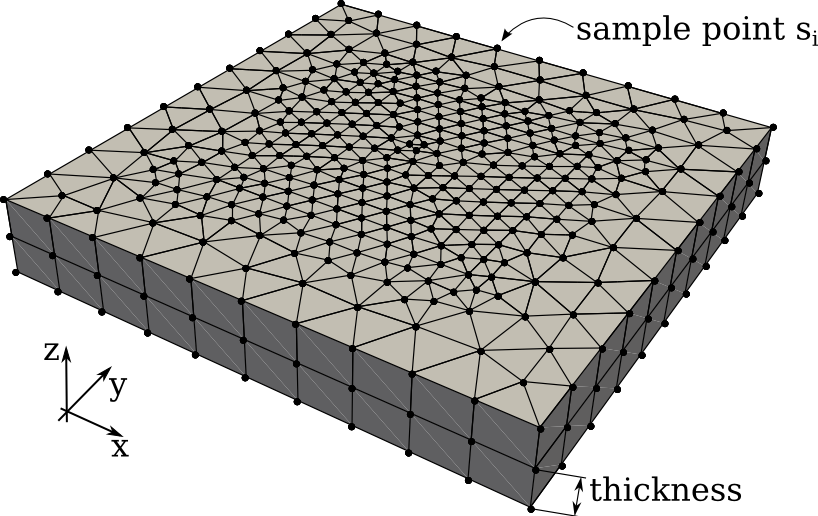
\includegraphics{graphics/samples_reduced.png}}
  }
  \caption{non-uniform sampling of active gain medium in 2 slices}
  \label{graphic:samples_reduced}
\end{figure}

The triangle mesh is extruded in direction of the vertical axis to form a
\emph{slice} of right prisms (Figure \ref{graphic:extruded_mesh}). This
slice is then duplicated several times, until the whole medium is divided into
prisms (Figure \ref{graphic:samples_reduced}).

\begin{figure}[H]
  \centerline{
    \resizebox{0.5\textwidth} {!} {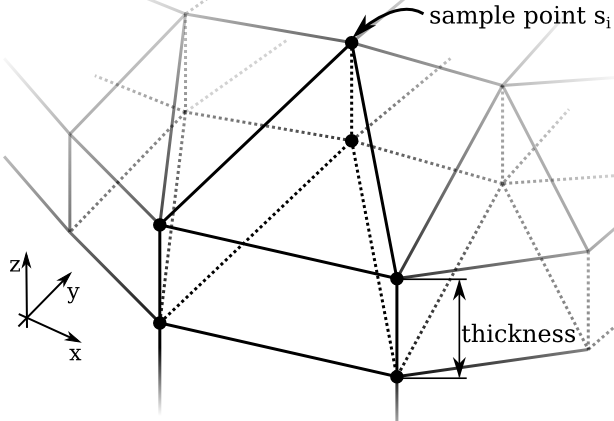
\includegraphics{graphics/delauny_4.png}}
  }
  \caption{extruded plane of triangles}
  \label{graphic:extruded_mesh}
\end{figure}

\subsection{Ray tracing}
\label{subsec:raytracing}

For calculating the amplification of a single ray from a position $r_{i,u}$ to a sample
point $s_i$, the ray is traced along its path through the prisms (see Figure
\ref{graphic:prism_propagation}). 

\begin{figure}[H]
  \centerline{
    \resizebox{0.5\textwidth} {!} {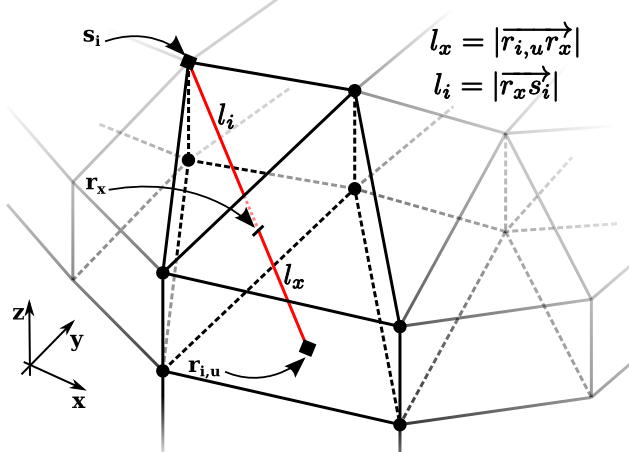
\includegraphics{./graphics/prism_propagation_4.png}}
  }
  \caption{propagation of a ray through the prism structure}
  \label{graphic:prism_propagation}
\end{figure}

Starting from point $r_{i,u}$ inside a prism, there are 5 possible intersection
planes with the ray. One plane for the top and bottom surfaces and one for each
of the 3 horizontal sides. Once the intersection plane is determined (the ray is
intersecting at point $r_x$), the next prism can be calculated based on the
knowledge about the mesh structure:

\begin{description}

  \item[horizontal side]
    the ray will remain in the same slice, but the next prism is based on a
    different triangle. This triangle is a \emph{neighbor} of the previous one.
    The relevant datastructure to determine the neighboring triangle is created
    during the Delauny triangulation in section \ref{subsec:meshSampling}.

  \item[top/bottom plane]
    if the ray is intersecting with the top or bottom plane of the prism, the
    next prism will be based on the same triangle as before, but in a different
    slice.

\end{description}

This process is iterated for each prism on the path between $r_{i,u}$ and the
desired sample point $s_i$. The intersections (like $r_x$) with prism surfaces
define line segments of a certain length $l_x$. These segments are used for the
gain calculation: For each prism $x$, the contribution to the gain is calculated
as a function of $l_x$:

\begin{equation}
\label{eq:partial_gain}
  partial\_gain(x) = 
  e^{N_{tot} \cdot (\beta_x \cdot (\sigma_e + \sigma_a) - \sigma_a)) \cdot l_x}
\end{equation}
where $\beta_x$ is the stimulus in the current
prism and $\sigma_e$, $\sigma_a$ are emission and absorption
values from a random wavelength over the polychromatic spectrum.

The gain for the whole ray can then be computed as

\begin{equation}
\label{eq:gain}
  gain(\overrightarrow{r_{i,u}s_i}) =  
  \frac{\prod^npartial\_gain(n)}{ |\overrightarrow{r_{i,u}s_i}|^2}  
\end{equation}



\subsection{Reflections}
\label{subsec:reflections}

\begin{figure}[H]
  \centerline{
    \resizebox{0.5\textwidth} {!} {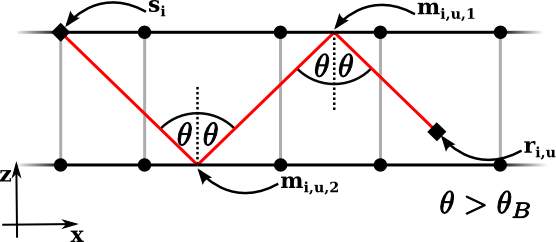
\includegraphics{./graphics/reflections_2.png}}
  }
  \caption{total internal reflections on the gain medium surface}
  \label{graphic:reflections_2D}
\end{figure}
\begin{figure}[H]
  \centerline{
    \resizebox{0.5\textwidth} {!} {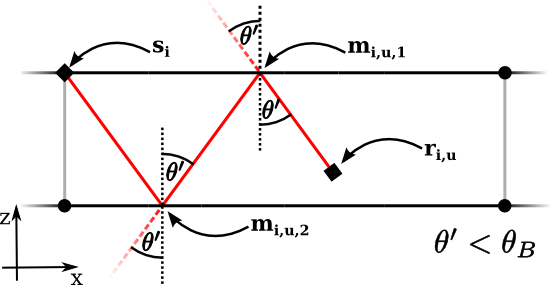
\includegraphics{./graphics/transmission1.png}}
  }
  \caption{reflections with partial transmission on the gain medium surface}
  \label{graphic:transmission_2D}
\end{figure}
In order to allow a more detailed simulation, the model is extended to include
reflections on the surface of the medium. The ray is split into multiple
separate sub-rays, each representing one part of the reflection (see Figure
\ref{graphic:reflections_2D}: $\overrightarrow{r_{i,u}m_{i,u,1}}$,
$\overrightarrow{m_{i,u,1}m_{i,u,2}}$, $\overrightarrow{m_{i,u,2}s_i}$).

On each of the reflection points, Brewster's angle $\theta_{B}$ is calculated to
estimate the \emph{initial gain} $g_i$ of a ray that is reflected at position
$x_i$:

\begin{equation}
\label{eq:gain_reflection}
  g_i = 
  \begin{cases}
    gain(\overrightarrow{x_{i-1}x_i}) & \text{if } \theta \ge \theta_{B}  \\
    gain(\overrightarrow{x_{i-1}x_i}) \cdot \gamma(x_i) & \text{if } \theta < \theta_{B}   
  \end{cases}
\end{equation}
Where $\gamma(x_i)$ is the fraction of the reflected energy (the reflectivity)
when the angle is too acute for total internal reflection, based on the surface
coating. $x_n$ refers to
either a mirror point $m_n$, $r_{i,u}$ or $s_i$.

The computation of all sub-rays comprises a significant overhead over the more
simplistic model with just a single ray, which necessitates the use of a high
performance algorithm.  The current implementation includes different refractive
indices as well as varying reflectivites for each Delaunay triangle. However,
only reflections on the upper and lower surface are supported, resulting in a
limited simulation that disregards lateral feedback. 
